\newif\ifieeeclass
\IfFileExists{IEEEtran.cls}{\ieeeclasstrue}{\ieeeclassfalse}
\ifieeeclass
\documentclass[10pt,journal,onecolumn,draftclsnofoot]{IEEEtran}
\else
\documentclass[11pt]{article}
\usepackage[margin=1in]{geometry}
\fi

\usepackage[T1]{fontenc}
\usepackage[utf8]{inputenc}
\usepackage{amsmath}
\usepackage{array}
\usepackage{booktabs}
\usepackage{float}
\usepackage{graphicx}
\usepackage{hyperref}
\usepackage{longtable}
\usepackage{multirow}
\usepackage{xcolor}
\usepackage{caption}
\usepackage{enumitem} % Added for list spacing optimization

% Reduce spacing in lists to save space
\setlist{nosep} 
\captionsetup[figure]{justification=centering,singlelinecheck=false}

\hypersetup{
    colorlinks=true,
    linkcolor=blue,
    urlcolor=blue,
    citecolor=blue
}

\newcolumntype{L}[1]{>{\raggedright\arraybackslash}p{#1}}
\newcolumntype{C}[1]{>{\centering\arraybackslash}p{#1}}
\newcolumntype{R}[1]{>{\raggedleft\arraybackslash}p{#1}}
\newcommand{\fitwidth}[1]{\resizebox{\linewidth}{!}{#1}}

\newcommand{\imgplaceholder}[2][0.9\linewidth]{%
  \framebox{\parbox{#1}{\centering
    \vspace{1cm}
    \textbf{Image Placeholder} \\
    \small\textit{#2}
    \vspace{1cm}
  }}%
}

\title{Homework 2 Report:\\ AI-Generated Text Detection, BERT Fine-Tuning, and Local LLM Adversarial Rewriting Analysis}
\author{Jiakai Zhong\\Student ID: 314831009}
\date{}

\begin{document}
\maketitle
\emergencystretch=2em

\begin{abstract}
This report summarizes Homework 2 for the course \textit{RNN and Transformer}. The homework studies AI-generated text detection on the \texttt{DAIGT V2} dataset and analyzes whether a local instruction-tuned large language model can rewrite human essays in a way that fools a trained detector. The full pipeline is built around a shared cleaned dataset and a fixed stratified train-validation split so that all experiments are directly comparable. Part 1 performs data cleaning, exploratory data analysis, and two TF-IDF plus logistic-regression baselines. Part 2 fine-tunes \texttt{bert-base-cased} and \texttt{bert-large-cased} under the same split and evaluation protocol. Part 3 applies \texttt{Meta-Llama-3-8B-Instruct} to rewrite essays and evaluates the rewritten outputs with the best detector. The main findings are as follows. First, the dataset already contains strong surface-level signals, so TF-IDF baselines achieve extremely high scores. Second, \texttt{bert-large-cased} is the best detector, but its gain over \texttt{bert-base-cased} is small relative to the extra training cost. Third, the local LLM rewriting attack completely fails in the tested setting: rewritten texts are not harder to detect, but instead become much more likely to be classified as AI-generated. This indicates that making a text more fluent, cleaner, and more stylistically uniform can itself become a strong detection cue.
\end{abstract}

\section{Assignment Objective and Experimental Setup}

\begin{itemize}
\item Course: \textit{RNN and Transformer}
\item Topic: AI-generated text detection and local LLM adversarial rewriting analysis
\item Dataset: \texttt{DAIGT V2} (Cleaned size: 44,864 samples)
\item Label definition: \texttt{0 = Human}, \texttt{1 = AI}
\item Shared split: stratified 80/20 train-validation split with \texttt{seed = 42}
\item Baseline models: \texttt{word bi-gram TF-IDF} and \texttt{char 3-5 gram TF-IDF} (+ LogisticRegression)
\item BERT detectors: \texttt{bert-base-cased} and \texttt{bert-large-cased}
\item Local generation model: \texttt{Meta-Llama-3-8B-Instruct}
\item Detector used in attack evaluation: \texttt{bert-large-cased}
\end{itemize}

The homework is organized into four parts:
\begin{enumerate}
\item Data cleaning, exploratory data analysis, and traditional baselines.
\item Fine-tuning and comparing \texttt{bert-base-cased} and \texttt{bert-large-cased}.
\item Evaluating local LLM rewriting attacks against the best detector.
\item Writing an integrated analysis report on performance, robustness, and failure cases.
\end{enumerate}

The key experimental principle is that all scripts share the same cleaned dataset and the same split file. Therefore, the baseline, BERT, and attack experiments are directly comparable and do not suffer from split inconsistency.

\section{Evaluation Metrics}

The report uses the following metrics:
\begin{align*}
\text{Accuracy} &= \frac{\text{correct predictions}}{\text{total samples}}, \quad
\text{Precision} = \frac{\text{TP}}{\text{TP} + \text{FP}}, \quad
\text{Recall} = \frac{\text{TP}}{\text{TP} + \text{FN}} \\
\text{F1} &= \frac{2 \cdot \text{Precision} \cdot \text{Recall}}{\text{Precision} + \text{Recall}}, \quad
\text{Attack Success Rate} = \frac{\text{rewritten texts predicted as Human}}{\text{number of rewritten texts}}
\end{align*}
\texttt{ROC-AUC} is the primary overall discrimination metric because it evaluates the ranking quality of the detector over all possible thresholds. For the adversarial attack experiment, the report also tracks the change in AI probability before and after rewriting.

\section{Part 1: Data Preparation and Exploratory Data Analysis}

\subsection{Data Cleaning and Shared Split}

The preprocessing steps applied to \texttt{train\_v2\_drcat\_02.csv}:
\begin{enumerate}
\item Keep only the \texttt{text} and \texttt{label} columns; convert text to string and strip spaces.
\item Remove null entries, empty strings, and exact duplicates based on the pair \texttt{(text, label)}.
\item Build a stratified 80/20 train-validation split with \texttt{seed = 42}.
\end{enumerate}

The cleaned dataset statistics are: Human: 27,367; AI: 17,497; Train: 35,891; Validation: 8,973.

\subsection{Main Descriptive Statistics}

\begin{table}[H]
\centering
\caption{Main descriptive statistics of the cleaned dataset}
\label{tab:eda_stats}
\small
\setlength{\tabcolsep}{5pt}
\begin{tabular}{@{}L{5.2cm}R{2.2cm}R{2.2cm}R{2.2cm}@{}}
\toprule
Statistic & Overall & Human & AI \\
\midrule
Sample count & 44,864 & 27,367 & 17,497 \\
Median word count & 359 & 388 & 334 \\
Median token length & 426 & 456 & 400 \\
Median vocabulary richness & 0.4436 & 0.4374 & 0.4531 \\
Truncation rate at 512 tokens & 0.2865 & 0.4034 & 0.1036 \\
\bottomrule
\end{tabular}
\end{table}

Vocabulary richness measures the proportion of distinct tokens within one essay (\(\frac{\text{unique tokens}}{\text{total tokens}}\)).

\subsection{EDA Figures and Interpretation}

The dataset is not fully balanced (more Human essays), necessitating stratified splitting. Human essays are generally longer, while AI essays are more concentrated in length. AI essays have a slightly higher median vocabulary-richness score, likely because Human essays often contain repeated ideas or casual phrasing that lowers the ratio.

% Grouped Figures for Space Saving
\begin{figure}[H]
\centering
\begin{minipage}{0.48\textwidth}
  \centering
  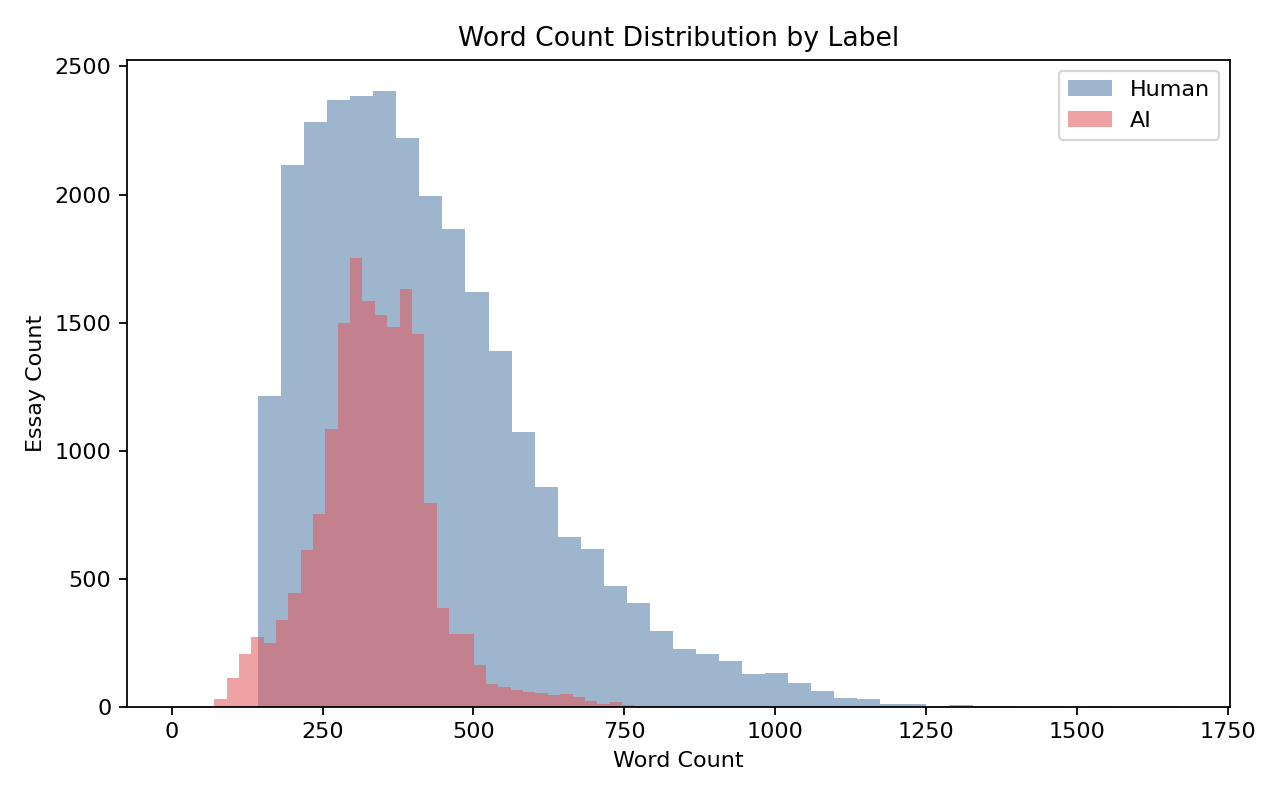
\includegraphics[width=\linewidth]{report_figures/eda_word_count_distribution.png}
  \caption{Word-count distribution}
  \label{fig:eda_word_count_distribution}
\end{minipage}\hfill
\begin{minipage}{0.48\textwidth}
  \centering
  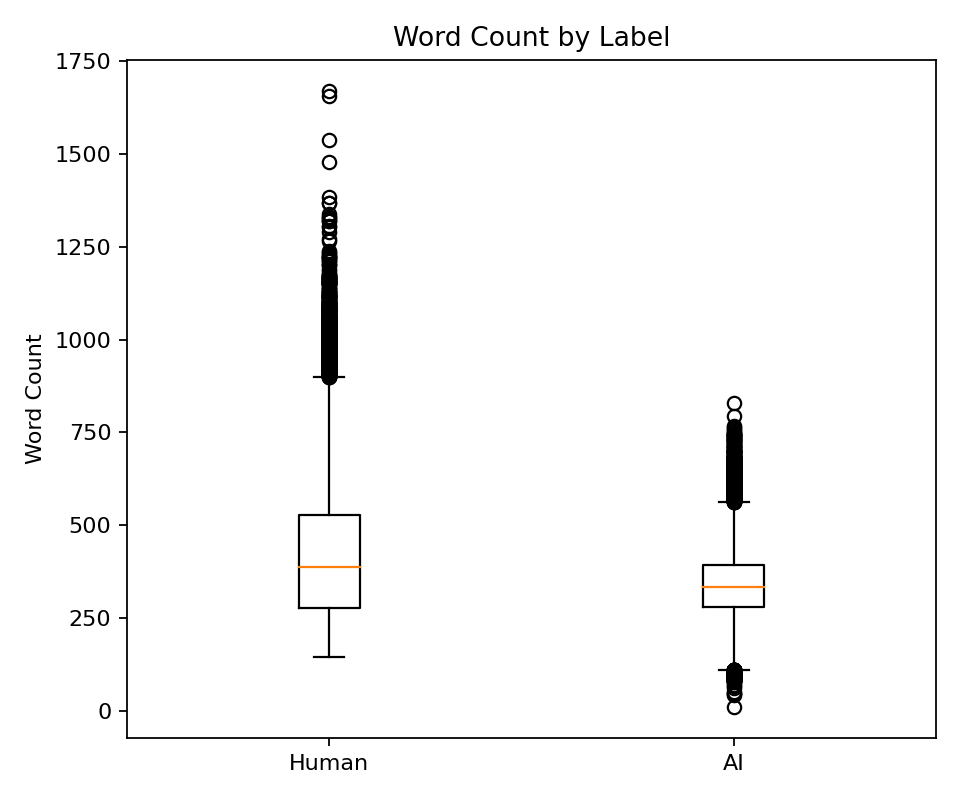
\includegraphics[width=\linewidth]{report_figures/eda_word_count_boxplot.png}
  \caption{Word-count boxplot}
  \label{fig:eda_word_count_boxplot}
\end{minipage}
\end{figure}

\begin{figure}[H]
\centering
\begin{minipage}{0.48\textwidth}
  \centering
  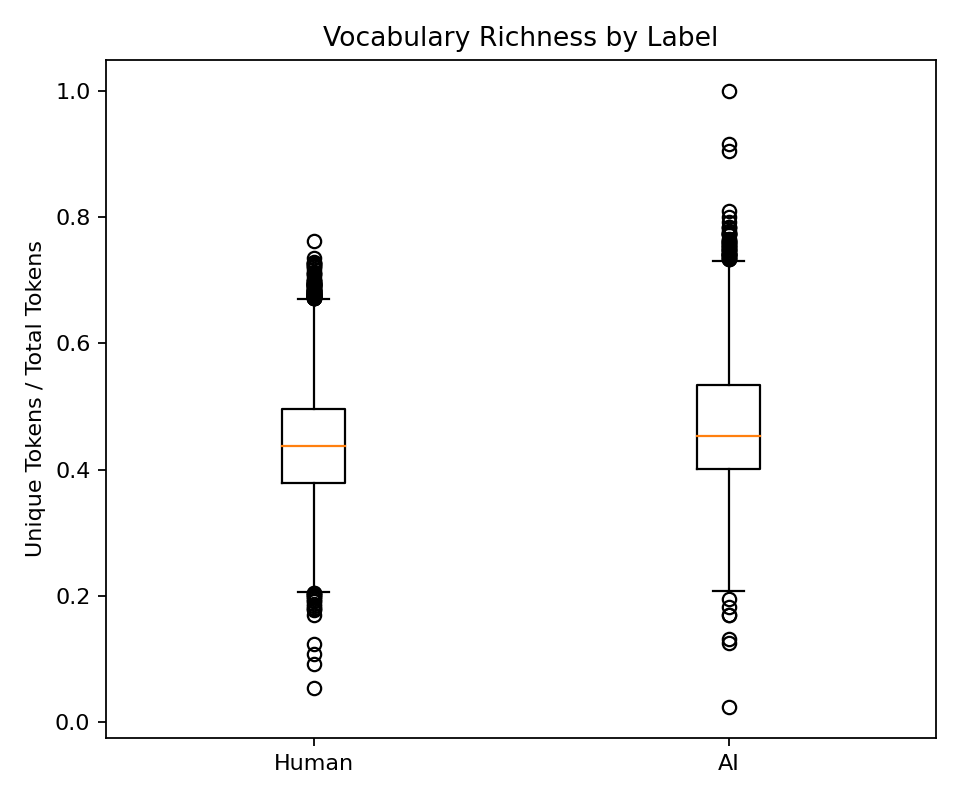
\includegraphics[width=\linewidth]{report_figures/eda_vocabulary_richness_boxplot.png}
  \caption{Vocabulary-richness boxplot}
  \label{fig:eda_vocabulary_richness}
\end{minipage}\hfill
\begin{minipage}{0.48\textwidth}
  \centering
  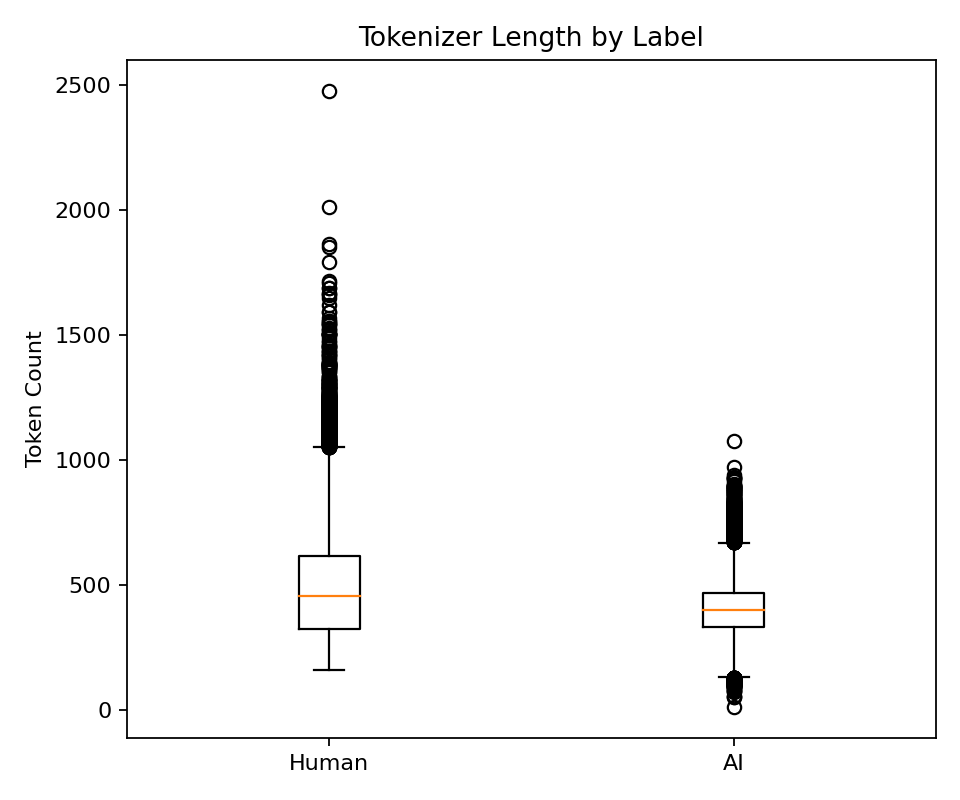
\includegraphics[width=\linewidth]{report_figures/eda_token_length_boxplot.png}
  \caption{Token-length boxplot (BERT)}
  \label{fig:eda_token_length}
\end{minipage}
\end{figure}

Under the \texttt{bert-base-cased} tokenizer, Human essays are much more likely to exceed 512 tokens, leading to a higher truncation rate.

\subsection{Statistical Test}

To verify observations, a Mann-Whitney U test was applied. All three p-values are far below 0.001, confirming statistical significance.

\begin{table}[H]
\centering
\caption{Mann-Whitney U test results}
\label{tab:eda_test}
\small
\setlength{\tabcolsep}{4pt}
\begin{tabular}{@{}L{4.0cm}R{1.8cm}R{1.8cm}R{2.0cm}R{2.5cm}@{}}
\toprule
Feature & Human Med. & AI Med. & p-value & Effect \\
\midrule
\texttt{word\_count} & 388.0000 & 334.0000 & 0.0000e+00 & 0.2456 \\
\texttt{vocabulary\_richness} & 0.4374 & 0.4531 & 4.2959e-190 & -0.1643 \\
\texttt{token\_length} & 456.0000 & 400.0000 & 0.0000e+00 & 0.2247 \\
\bottomrule
\end{tabular}
\end{table}


\section{Part 1: TF-IDF Baseline}

Two baselines were used: \texttt{word bi-gram TF-IDF + LR} and \texttt{char 3-5 gram TF-IDF + LR}. Both baselines are extremely strong, with the word-level baseline slightly outperforming the char-level one.

\begin{table}[H]
\centering
\caption{Overall TF-IDF baseline results}
\label{tab:baseline_overall}
\small
\setlength{\tabcolsep}{5pt}
\begin{tabular}{@{}L{4.0cm}R{1.8cm}R{1.8cm}R{1.8cm}R{1.8cm}R{1.8cm}@{}}
\toprule
Model & Accuracy & Precision & Recall & F1 & ROC-AUC \\
\midrule
Word TF-IDF + LR & 0.9927 & 0.9991 & 0.9822 & 0.9906 & 0.9992 \\
Char TF-IDF + LR & 0.9920 & 0.9973 & 0.9822 & 0.9897 & 0.9990 \\
\bottomrule
\end{tabular}
\end{table}

% Grouped Class-wise reports
\begin{table}[H]
\centering
\small
\begin{minipage}{0.48\textwidth}
  \centering
  \caption{Word TF-IDF Class Report}
  \label{tab:baseline_word_class}
  \fitwidth{%
  \begin{tabular}{@{}lcccc@{}}
  \toprule
  Class & Prec. & Recall & F1 & Supp. \\
  \midrule
  Human & 0.988 & 0.999 & 0.994 & 5474 \\
  AI & 0.999 & 0.982 & 0.990 & 3499 \\
  \bottomrule
  \end{tabular}%
  }
\end{minipage}\hfill
\begin{minipage}{0.48\textwidth}
  \centering
  \caption{Char TF-IDF Class Report}
  \label{tab:baseline_char_class}
  \fitwidth{%
  \begin{tabular}{@{}lcccc@{}}
  \toprule
  Class & Prec. & Recall & F1 & Supp. \\
  \midrule
  Human & 0.988 & 0.998 & 0.993 & 5474 \\
  AI & 0.997 & 0.982 & 0.989 & 3499 \\
  \bottomrule
  \end{tabular}%
  }
\end{minipage}
\end{table}

% Grouped ROC Curves
\begin{figure}[H]
\centering
\begin{minipage}{0.48\textwidth}
  \centering
  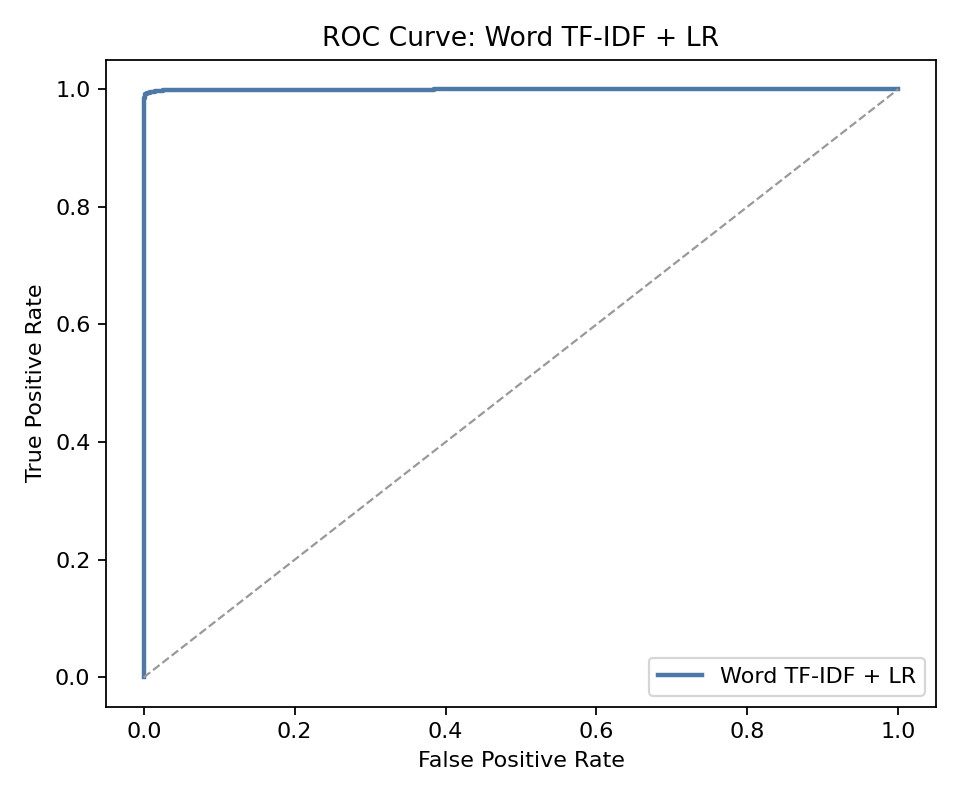
\includegraphics[width=\linewidth]{report_figures/baseline_roc_word_tfidf.png}
  \caption{ROC (Word TF-IDF)}
  \label{fig:baseline_roc_word}
\end{minipage}\hfill
\begin{minipage}{0.48\textwidth}
  \centering
  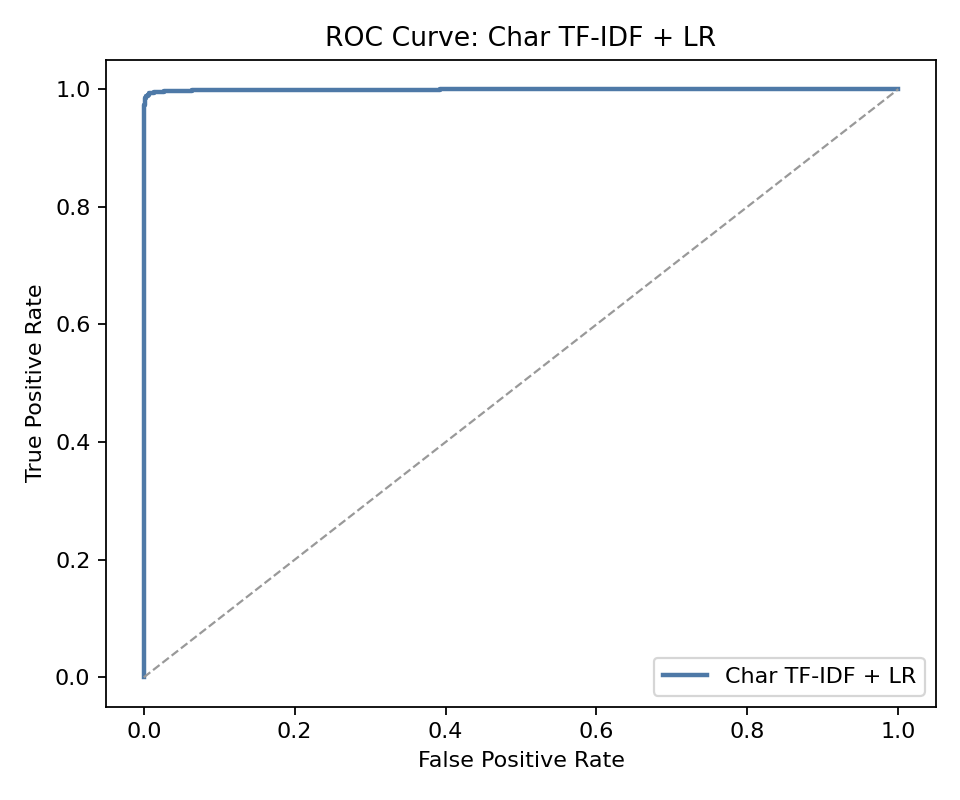
\includegraphics[width=\linewidth]{report_figures/baseline_roc_char_tfidf.png}
  \caption{ROC (Char TF-IDF)}
  \label{fig:baseline_roc_char}
\end{minipage}
\end{figure}

% Grouped Confusion Matrices
\begin{figure}[H]
\centering
\begin{minipage}{0.48\textwidth}
  \centering
  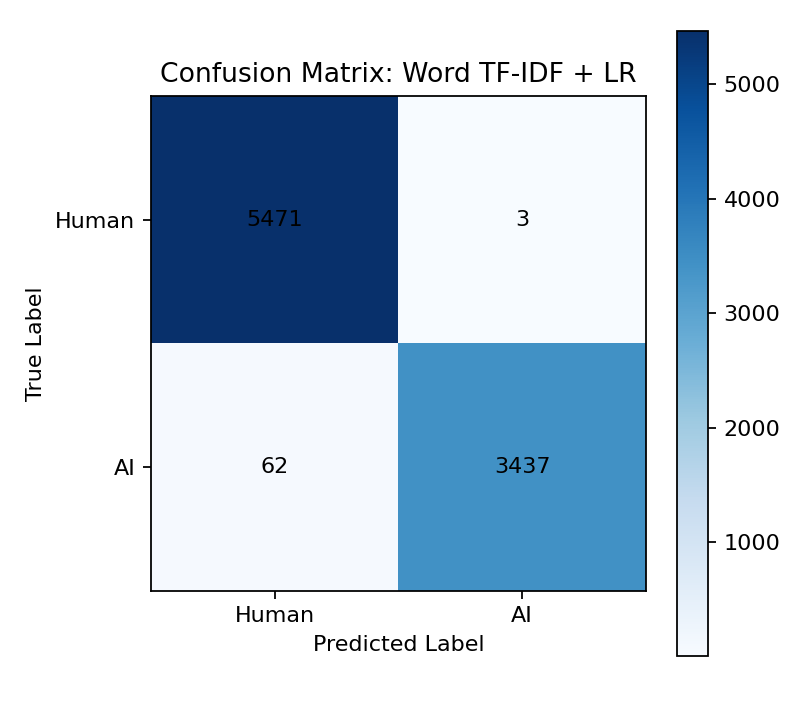
\includegraphics[width=\linewidth]{report_figures/baseline_confusion_word_tfidf.png}
  \caption{Confusion Matrix (Word)}
  \label{fig:baseline_conf_word}
\end{minipage}\hfill
\begin{minipage}{0.48\textwidth}
  \centering
  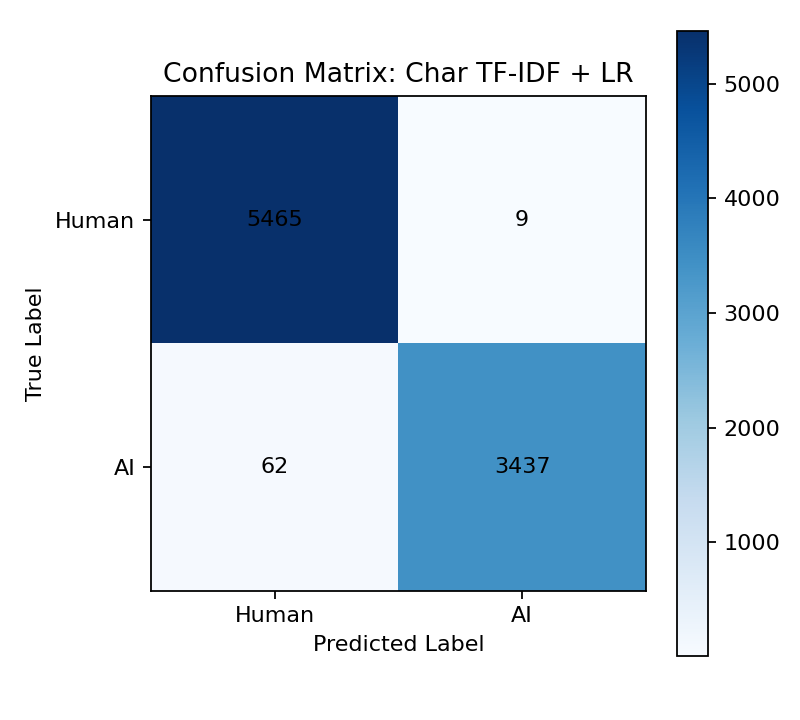
\includegraphics[width=\linewidth]{report_figures/baseline_confusion_char_tfidf.png}
  \caption{Confusion Matrix (Char)}
  \label{fig:baseline_conf_char}
\end{minipage}
\end{figure}

The very high baseline is not caused by data leakage (0 exact text overlap between train and validation). The strong performance is explained by the dataset containing strong lexical, phrasal, and structural cues.


\section{Part 2: BERT Fine-Tuning and Comparison}

Two BERT detectors (\texttt{base} and \texttt{large}) are compared with \texttt{max\_length = 512}, effective batch size = 32, mixed-precision training, and shared split. \texttt{bert-large-cased} also uses gradient checkpointing.

\begin{table}[H]
\centering
\caption{BERT fine-tuning results across two random seeds}
\label{tab:bert_results}
\small
\setlength{\tabcolsep}{5pt}
\begin{tabular}{@{}lccccc@{}}
\toprule
Model & Seed & Accuracy & F1 & ROC-AUC & Runtime (s) \\
\midrule
\texttt{bert-base-cased} & 42 & 0.9914 & 0.9890 & 0.9996 & 541.80 \\
\texttt{bert-base-cased} & 7 & 0.9915 & 0.9891 & 0.9996 & 388.61 \\
\texttt{bert-large-cased} & 42 & 0.9957 & 0.9945 & 0.9997 & 1460.69 \\
\texttt{bert-large-cased} & 7 & 0.9932 & 0.9913 & 0.9997 & 1419.50 \\
\bottomrule
\end{tabular}
\end{table}

\begin{figure}[H]
\centering
\begin{minipage}{0.48\textwidth}
  \centering
  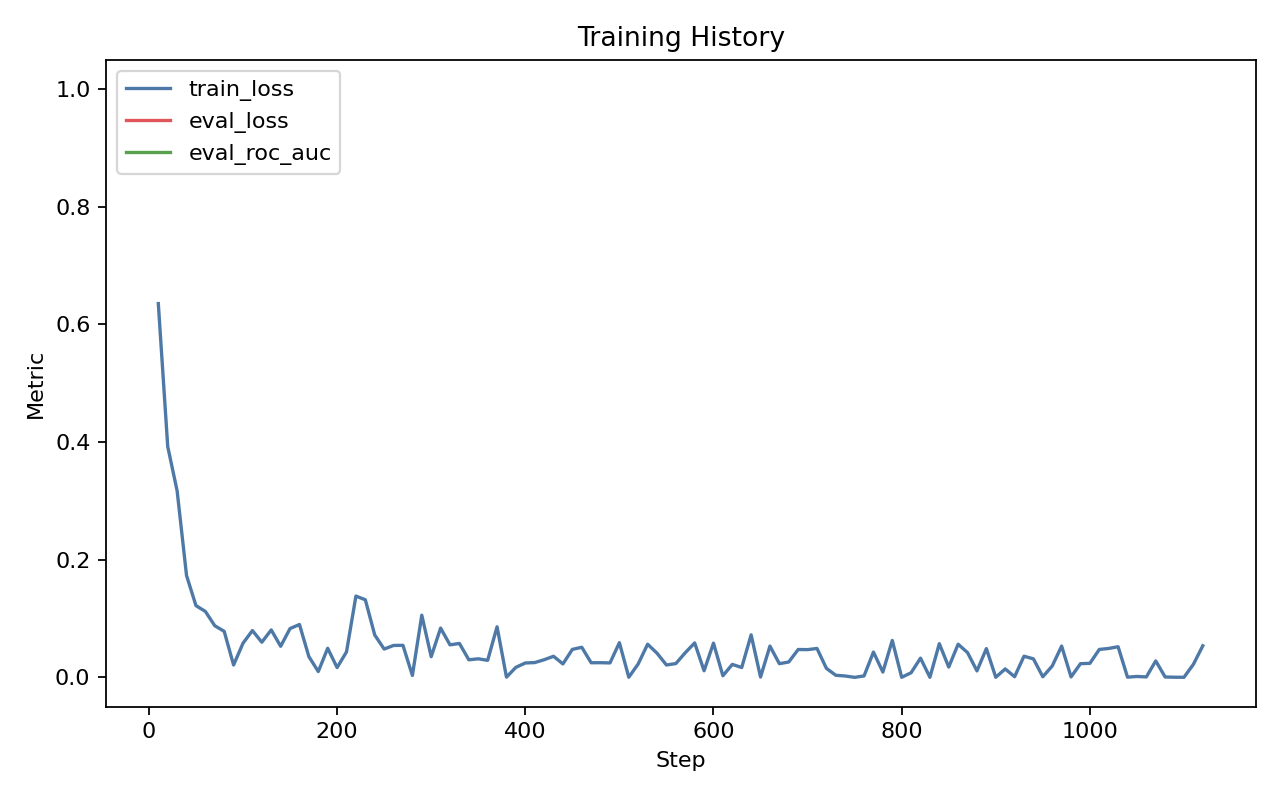
\includegraphics[width=\linewidth]{report_figures/bert_base_training_history.png}
  \caption{Training history (\texttt{base}, seed 42)}
  \label{fig:bert_base_history}
\end{minipage}\hfill
\begin{minipage}{0.48\textwidth}
  \centering
  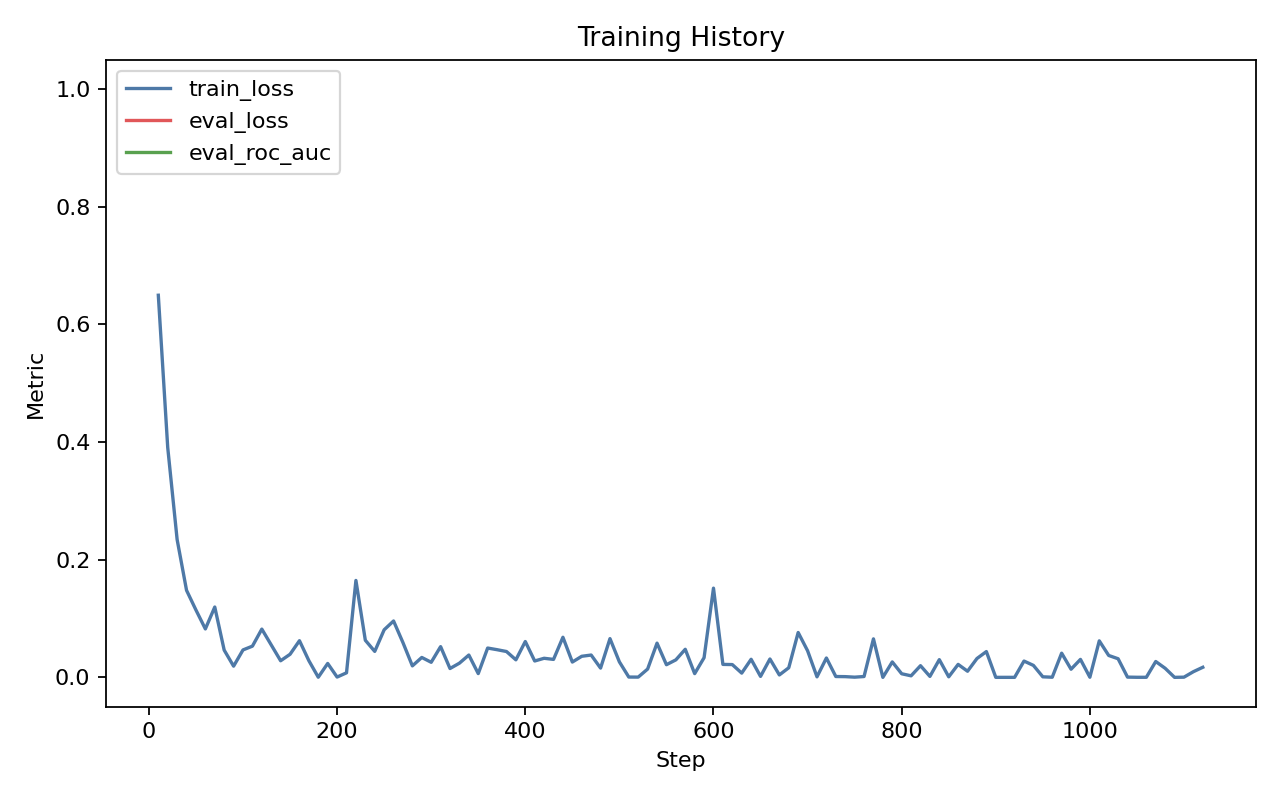
\includegraphics[width=\linewidth]{report_figures/bert_large_training_history.png}
  \caption{Training history (\texttt{large}, seed 42)}
  \label{fig:bert_large_history}
\end{minipage}
\end{figure}

\textbf{Analysis:} \texttt{bert-large-cased} is consistently better, but the gain is small while the runtime cost is roughly 2.6x to 3.7x higher. Despite the high truncation rate for Human texts, the detectors perform extremely well, suggesting the first 512 tokens already carry strong discrimination cues.


\section{Part 3: Local LLM Adversarial Rewriting Attack}

Validation essays correctly classified as Human are rewritten by \texttt{Meta-Llama-3-8B-Instruct} to test bypass capability against the best \texttt{bert-large-cased} detector. 

\subsection{Attack Results (Round 1 \& Stealth Round)}

In the first round using \texttt{student\_voice} and \texttt{natural\_imperfect} prompts (10 source, 20 attack samples), the attack success rate was 0.0. The mean rewritten AI probability shot up from 0.000115 to 0.999952.

The second "stealth" round used a conservative prompt set (\texttt{minimal\_edit}, \texttt{messy\_student}, \texttt{lighter\_revision}) with 30 attack samples. The overall success rate remained 0.0.

\begin{table}[H]
\centering
\caption{Prompt-level stealth attack results}
\label{tab:attack_prompt}
\small
\begin{tabular}{@{}lc@{}}
\toprule
Prompt & Mean rewritten AI probability \\
\midrule
\texttt{minimal\_edit} & 0.999888 \\
\texttt{messy\_student} & 0.999979 \\
\texttt{lighter\_revision} & 0.999982 \\
\bottomrule
\end{tabular}
\end{table}

\begin{figure}[H]
\centering
\begin{minipage}{0.48\textwidth}
  \centering
  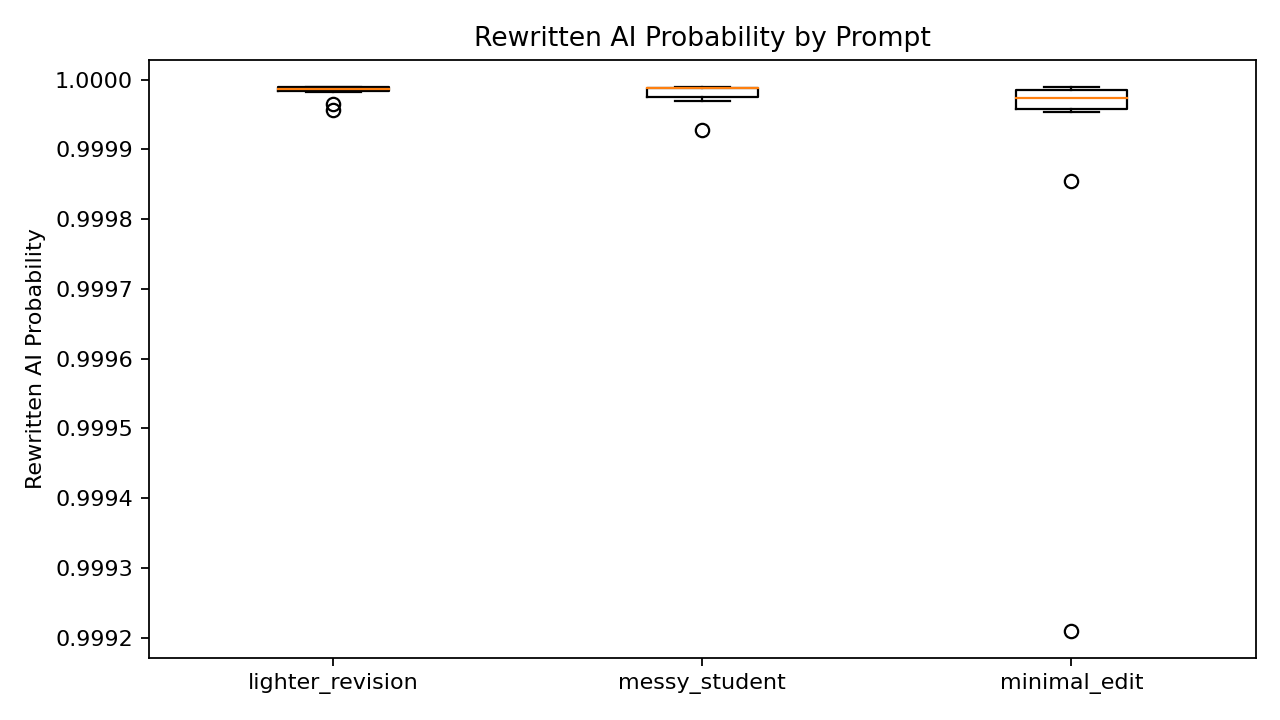
\includegraphics[width=\linewidth]{report_figures/attack_rewritten_ai_prob_by_prompt.png}
  \caption{Rewritten AI prob (stealth)}
  \label{fig:attack_rewritten_prob}
\end{minipage}\hfill
\begin{minipage}{0.48\textwidth}
  \centering
  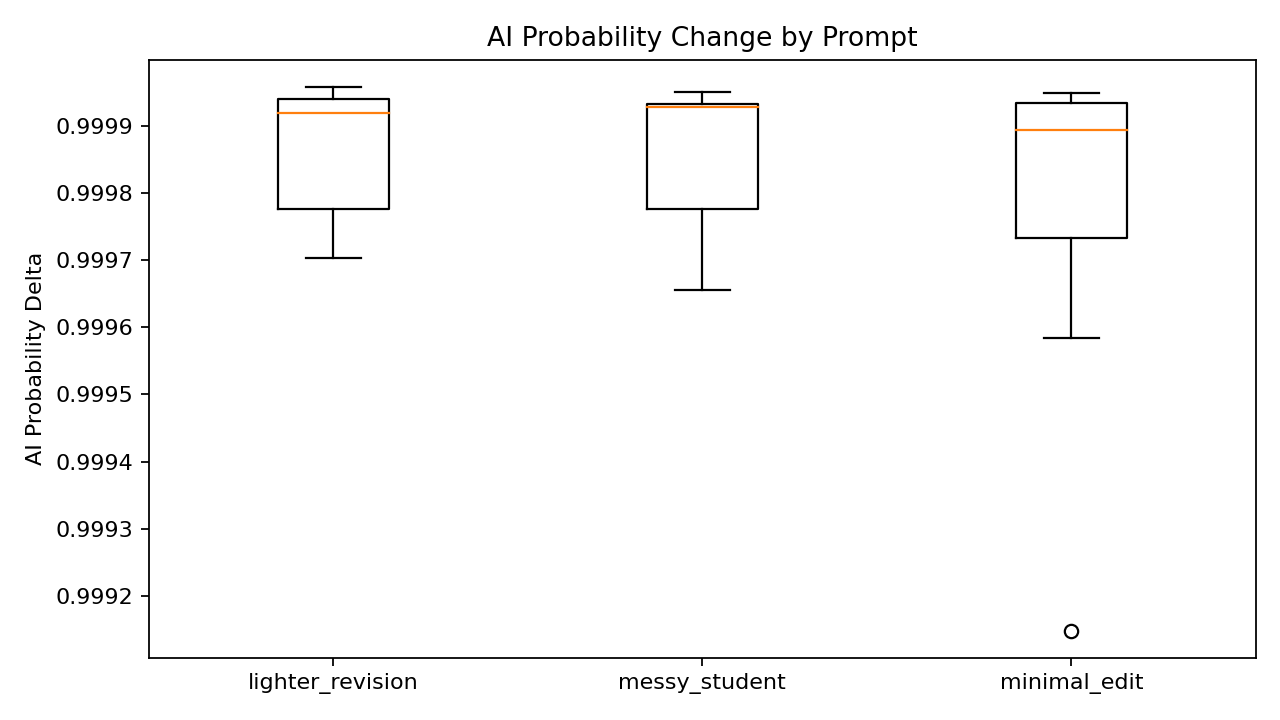
\includegraphics[width=\linewidth]{report_figures/attack_ai_prob_delta_by_prompt.png}
  \caption{AI-prob increase after rewriting}
  \label{fig:attack_delta}
\end{minipage}
\end{figure}

The attack-success figure is omitted here because all prompts have a success rate of 0.0. The original plot is therefore visually blank, and the text description is more informative than including an empty figure.


\section{Part 4: Analysis Report}

\subsection{Integrated Findings and Baseline Reasoning}
The Human and AI texts in \texttt{DAIGT V2} are strongly separable. The TF-IDF baselines are so strong that BERT's additional gain is limited. Because the word baseline slightly outperforms the char baseline, the strong performance is better explained by lexical choice, phrase usage, and discourse regularity, rather than shallow character artifacts. 

\subsection{Near-Success Attack Cases \& Why the Attack Fails}
Although no attack succeeded, cases like \texttt{row\_id=22196} or \texttt{6587} under \texttt{minimal\_edit} show that the Llama rewrite improves fluency, corrects spelling, and reorganizes the text into a more regular structure. 

The attack failure is driven by three main factors:
\begin{itemize}
\item Llama-3 tends to make the text cleaner and smoother, rather than preserving genuine human noise.
\item The original irregularities in high-confidence Human samples are precisely the features that help the detector classify them as Human.
\item The detector exploits overall stylistic consistency; once the rewrite becomes too regular, it is easily identified as AI.
\end{itemize}

\subsection{Limitations and Future Directions}
Limitations include relying on a single instruction-tuned model, using prompt engineering rather than constrained decoding, and evaluating with a fixed 512-token BERT window. Future work could explore rewriting methods that deliberately preserve authentic human noise.

\section{Discussion and Reflection}
\begin{itemize}
\item Strong Human-AI separability in \texttt{DAIGT V2} explains why traditional models perform near the ceiling.
\item Fluency improvement does not equal stealth; a cleaner rewrite is often easier to detect.
\item Human-like irregularity is not merely noise---it is often the crucial evidence of genuine human authorship.
\end{itemize}

\end{document}
